\ifdefined\included
\else
\setcounter{chapter}{5} %% Numéro du chapitre précédent ;)
\dominitoc
\faketableofcontents
\fi

\chapter{Estimating communication feasibility and cost at task planning}
\chaptermark{Estimating communication at task planning}
\minitoc

The contribution presented in this chapter is excerpted from our work, published in the proceedings of the ICSR 2020 conference~\cite{buisan_2020_human}. In this manuscript, the contribution is more detailed and discussed. In the continuity of the previous, the presented work has been achieved in collaboration with Guilhem Buisan. While his focus was on task planning, mine was on the link between the knowledge base as an ontology and the task planner. In this thesis, we will deepen this link and discuss possible improvements to the one initially presented.

\section{Introduction}

It is well established that a key aspect of the success of collaborative tasks is based on clear and fluent communication grounded in the context of the interaction. In the Natural Language Processing (NLP) research field and by extension in the Human-Robot Interaction (HRI) field, it has been divided into two dual problems~\cite{tellex_2020_robots}. On one hand, the Natural Language Understanding (NLU) aims the robot to interpret and grounds human's utterances with regard to the current situation and to react according to it~\cite{brawer_2018_situated}. In another hand, the Natural Language Generation (NLG) aims the robot to produce language. It could either be to ask for help~\cite{tellex_2014_asking}, to align knowledge~\cite{devin_2016_implemented}, or to explain its decision to its partner~\cite{roncone_2017_transparent}.

In the previous chapter, we have introduced an algorithm able to generate the content of a referring expression. Such contribution thus falls in the NLG problem. Considering the REG as an action that can be performed by the robot means that the robot could plan such communication in terms of \textbf{when} and \textbf{what} to communicate. While the "when" is directly handled by the task planner, the "what" is provided by the REG. However, the REG does not only provide the content but is also able to state if such communication is feasible or not and give information about its cost depending on the number of relations to communicate. Because the REG algorithm work on a knowledge base representing the current state of the environment, maintaining a comparable representation of the environment for the future states of the task (as it is done in symbolic task planning) would allow the robot to estimate the \textbf{feasibility} and the \textbf{cost} of the verbal communication actions all along with a task.

With these two pieces of information, a task planner could compare verbal communication with one another, compare with other means of communication, minimize the overall communication complexity, and prevent some plan failures. This approach to estimating the communication at task planning can be compared to the one proposed in~\cite{lallement_2016_symbolic}. In the latter, motion actions were evaluated at task planning to estimate their feasibility, costs, and indirect effects. With both approaches, the symbolic plans can be optimized and can be more reliable in preventing execution failures and thus the need for reparation.


\begin{figure}[t!]
\centering
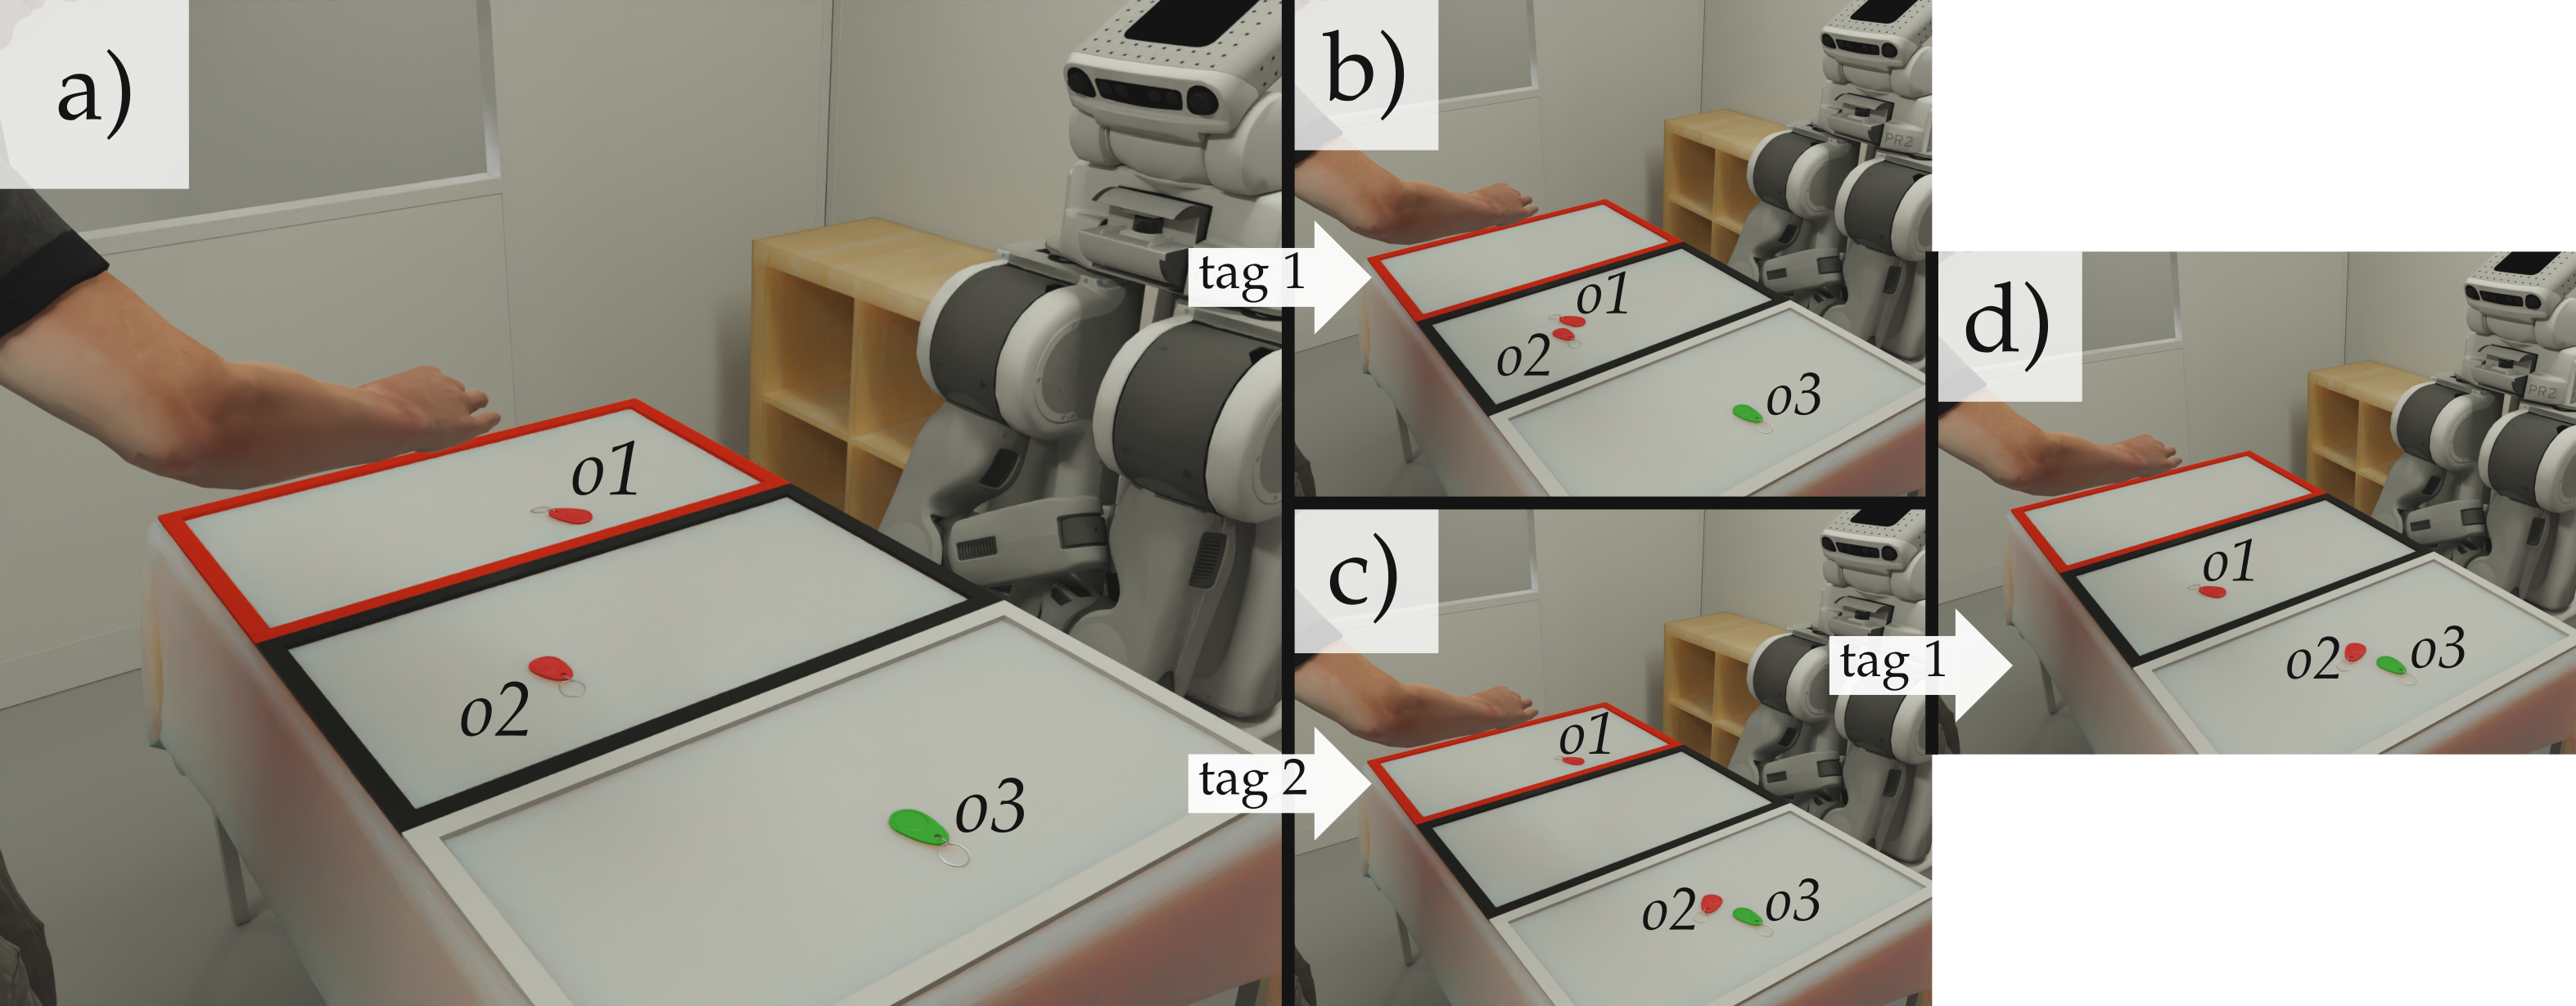
\includegraphics[width=\textwidth]{figures/chapter5/intro/intro.png}
\caption{\label{fig:chap5_intro} A Human-Robot collaborative task with three colored areas and three RFID tags (situation a). The robot has to explain to its human partner to put the tag \textit{o1} in the black area and the tag \textit{o2} in the white area, to reach the situation d. The objects identifiers' are only known to the robot.
If all the communications of the task are not planned ahead, a deadlocked situation could appear if the robot first asks to move the tag \textit{o1} before \textit{o2} (situation b).}
\end{figure}

To better understand the advantage to consider the communication at task planning, consider the situations of Figure~\ref{fig:chap5_intro}. The robot has to arrange RFID tags on three areas on a table. The robot can identify them with their unique id but being too small, it can not grasp them. On the contrary, the human partner can not identify them uniquely but can grasp them. For this example, we also assume that the robot cannot point to the tags. The robot must therefore communicate the successive actions that the human will have to perform to go from the inial configuration (\ref{fig:chap5_intro} a) to the goal configuration (\ref{fig:chap5_intro} d). Between both configurations, only the tags \textit{o1} and \textit{o2} have to be moved. The tag \textit{o1} has to be move from the red area to the black and \textit{o2} from the black area to the white. While the tag \textit{o3} can be referred to unambiguously thanks to its color, the two others can not. However, they can be referred thanks to the area they are in (e.g. \textit{"the tag is the red area"}).

If the content of the communications is only refined at execution, two equivalent solutions can be planned (\ref{fig:chap5_intro} sequence a-b-d and a-c-d). At execution, the first solution begins by asking the human to move \textit{o1} in the black area resulting in the instruction \textit{"take the tag that is in the red area and put it in the black area"}. In this new situation where both red tags are now in the black area (Figure~\ref{fig:chap5_intro}b). The robot has no way to designate the tag \textit{o2} without ambiguity. Hence, the task is blocked\footnote{The robot could use spatial relation like right, left, or the closest to me. However, the generation of such RE is not an easy job and the understanding of it neither. Even if the situation is not really blocked, the required communication can be complex. }. Estimating the communication feasibility and cost during the planning process would result in the second possible solution. The robot first ask to move the tag \textit{o2} (Fig.~\ref{fig:chap5_intro} c) and then the tag \textit{o1} (Fig.~\ref{fig:chap5_intro} d). If the robot could have pointed, the deadlock of the first solution can be avoided with a pointing action and nevertheless, thanks to the communication cost estimation, the least expensive solution can be selected\footnote{Plenty of other solution could exist but depend on the robot capability. Giving the two instructions in the initial state before the human act solve also the problem for example. Nevertheless, if the robot cannot compare these different solutions regarding its current capability, non-desirable situations could still appear.}.

The main contribution presented in this chapter is an approach to \textbf{estimate the communication feasibility and cost at task planning}. It implies a fine \textbf{link between a planner and an ontology} to estimate communication grounding in the future estimated state of the environment.

First, we briefly review the literature concerning the task planning problem and discuss the issues we aim to tackle. Then we, give an overview of the involved components with a focus on the task planner while the others have been detailed in the previous chapters. We then present how the fine integration of the components allows us to take estimation the communication at task planning and discuss possible improvement. We end this chapter with three case studies, to show how this approach can be used to prevent deadlocked situations at execution, how it can reduce the global communication complexity during a Human-Robot collaborative task and how it can be used to balance between different communication means.

\section{Related work: The need to plan communication}


\section{The involved components}

\subsection{The Hierarchical Task Planner}

\subsection{The semantic knowledge base}

\subsection{The Referring Expression generator}


\section{Integrating task and communication planners}

\subsection{The representation of the communication action}

\subsection{Maintaining the right knowledge base, at the right time}


\section{Results}

\subsection{Prevent execution dead-end}

\subsection{Reduce the overall communication complexity}

\subsection{Compare with other communication means}